\documentclass[times, 10pt,twocolumn]{article} 
\usepackage{latex8}
\usepackage{times}
\usepackage{amsmath}
\usepackage{amsthm}
\usepackage{graphicx}
\usepackage{url}
\usepackage[utf8x]{inputenc}
\usepackage[T1]{fontenc}
\usepackage{color}
\usepackage{subfig}

\newtheorem{theorem}{Theorem}[section]

\newcommand{\comentario}[1]{}
\newcommand{\superscript}[1]{\ensuremath{^{\textrm{#1}}}}
\newcounter{notecounter}
\newcommand{\nota}[1]{\addtocounter{notecounter}{1}{\textcolor{red}{[nota
      \arabic{notecounter}: #1]}}}

\newcommand{\gnota}[1]{
  \addtocounter{notecounter}{1}
  \vspace{.5cm}
  \framebox{
    \begin{minipage}{0.95\linewidth}
      \textbf{nota \arabic{notecounter}:} #1
    \end{minipage}
  }\vspace{.5cm}}

\newcommand{\simul}{\textbf{Simul}} % Que criatividade. Mudar esse
% nome depois, urgente

\author{George Lima, Alexandre Passos, José Augusto Matos Santos}
\title{Hard Reservation vs Soft Reservation for soft real-time systems}

\begin{document}
\maketitle

\begin{abstract}

  When scheduling soft real-time tasks it is usually a good idea to
  reserve fractions of the total bandwidth to each task (or task
  group). This reservation might be either \textbf{hard}, when under
  no circumstances a task might use some extra bandwidth, or
  \textbf{soft}, if there are some situations when it is allowed to do
  so. Usually, specially in the context of on-line adaptative systems,
  hard reservation is perceived to be more predictable, stricter and
  allowing faster adaptation. In this paper we argue that, perhaps
  surprisingly, allowing tasks to use some idle bandwidth shouldn't
  hurt. To clarify our arguments we present the results of a few
  experiments performed on real-life and syntetic data sets using hard
  and soft variations of CBS, a commonly used reservation-based
  server.
  
\end{abstract}

\section{Introduction}
\label{sec:introduction}

In reservation-based scheduling of soft real-time tasks, each task is
allowed at most a given fraction of the total processor time. There
are two broad approaches to using said fraction: \textbf{hard} and
\textbf{soft} reservation. In a hard reservation framework each server
is allowed a given fraction of the total processing time, and in no
ocasion can use more than that fraction. If in some circumstances, a
pending task that has overrun its budget is allowed to use idle
processing time, then the reservation is said to be soft\nota{colocar
  referência da definição}. It is commonly acknowledged that a system
based on hard reservation is more predictable, if not more efficient,
than a system based on soft reservation. In this paper we present a
simulation environment for becnhmarking both reservation mechanisms
and experimental results in this environment that fail to show any
significant benefit either in predictability or in performance.

\subsection{Related work}
\label{sec:related-work}

In a paper on QoS management thourgh adaptive reservations
\cite{abeni.ea05:qos}, Abeni et al use a hard reservation approach to
help adaptivity. The need for such a restriction on the reservation
will be studied \nota{colocar um experimento com hard e soft
  corretamente dimensionados e variância maior/menor pra ver o que
  acontece} later in this paper.

\subsection{Contributions of this paper}
\label{sec:contr-this-paper}

The main contribution of this paper is putting into perspective the
perceived characteristics of hard reservation. There is a lack in
literature of experiments in a fair environment that measure
objectively the possible benefits and costs of using hard and soft
reservation in a given system.

\section{Analytical characteristics}
\label{sec:analyt-char}

In \cite{buttazzo05:soft}, hard reservation is introduced as a way of
proving schedulability of a given task set using a CBS server with a
hard reservation rule. It is done o by means of the following theorems:

\begin{theorem}
  Given a CBS server with the hard reservation rule, and with
  parameters $(Q,P)$, if $k =
  \left\lceil\frac{t-(P-Q)}{P}\right\rceil$, the partition with the
  maximum delay that it can generate has the following least supply
  function $S^*(t)$:
  \[ S^*(t) = \left\{ \begin{array}{ll}
      0 & \text{if}\ t \in [0,P-Q] \\
      (k-1)Q & \text{if}\ t \in (kP - Q, (k+1)P-2Q) \\
      t-(k+1)(P-Q) & \text{otherwise.}
    \end{array}\right.
  \]
\end{theorem}

\begin{theorem}
  Let $A$ be set of periodic or sporadic tasks
  $\{\tau_1,\ldots,\tau_n\}$, with $\tau_i = (C_i,T_i,D_i)$, where
  $C_i$ is the worst-case computation time, $T_i$ is the task period
  and $D_i$ is the relative deadline. This task set is schedulable by
  EDF scheduling algorithm on a resource partition with least supply
  function $S^*(t)$ if and only if:
  \[
  \forall 0 < t \leq 2H : dbf(t) \leq S^*(t)
  \]
  where $H = lcm(T_1,\ldots,T_n)$ is the hyperperiod of A and $dbf(t)$
  is the processor demand bound function, defined as
  \[
  dbf(t) = \sum_{i=1}^n
  \left(\left\lfloor\frac{t-D_i}{T_i}\right\rfloor + 1\right)C_i.
  \]
\end{theorem}

For a proof of these results, see \cite{buttazzo05:soft}.

Interestingly, these theorems can be extended to a soft reservation
framework. Intuitively, if a given task set is schedulable on a hard
cbs server, it means that if the server budget ever runs out when
executing a task from that task set, the task still has time to finish
before its deadline. Since the total computation time available for a
given server deadline is the same under both soft and hard reservation
and no tasks from the original task set are discarded, any task set
schedulable with the hard reservation rule is schedulable with the
soft reservation rule. \nota{formalizar essa prova}


\section{Simulation environment}
\label{sec:simul-envir}

To perform the experiments presented in this paper we implemented
\simul{}, a simple python-based simulator for real-time scheduling
algorithms. Its source code, the data files used in this paper and
instructions to reproduce our results are available in
\url{http://github.com/jamsjr/hard-versus-soft/tree/master}. \simul{}
implements a basic EDF scheduler and, on top of it, runs both hard
real-time periodic tasks and bandwidth sharing servers. These servers
can be either traditional CBS servers \cite{abeni.ea98:integrating} or
a hard reservation adaptation of the CBS algorithm, as described in
\cite{buttazzo05:soft}. Soft real-time tasks running on these servers
either have their execution times sampled from a probability
distribution or follow traces generated from a modified version of
mplayer that reports the start time and decoding cost for each frame
in a high-definition video running on a XXX\nota{pegar info do pc de
  eduardo}.

All the simulations performed in this paper share a common
environment. There is a hard real-time task running in the background,
with fixed period, execution costs and deadline. There is also one
soft real-time server (with hard or soft reservation) running tasks
from either the video trace or with costs drawn from a normal
distribution. All tasks considered are periodic, or approximately
periodic. Some other aspects of the simulation, though, are variable,
and it is our objective to understand how they influence the behavior
of soft or hard reservation.

\subsection{Controled variables}
\label{sec:controled-variables}

In our simulations we studied the possible effects of the given
variables:
\begin{itemize}
\item any \textbf{expired tasks} (tasks that ran over their deadlines)
  might be discarded or not;
\item the \textbf{execution costs} can be either from a real-life
  trace from a movie (shown in figure \ref{fig:plot-trace-eve}) or
  synthetic and normally distributed (seen in figure
  \ref{fig:plot-trace-normal});
\item when the execution costs are synthetic, their \textbf{variance}
  determines how much they stray from their expected value;
\item there might be \textbf{system idle time} or there might not;
\item the \textbf{server load} might be too high---meaning not all
  tasks can finish in the expected time---, correct---meaning all
  tasks should finish in the expected time---, or too low---meaning
  there will be substantial idle time in the server.
\end{itemize}

\begin{figure*}[t]
  \centering
  \subfloat[Execution costs for the trace of 'eve'.]{
    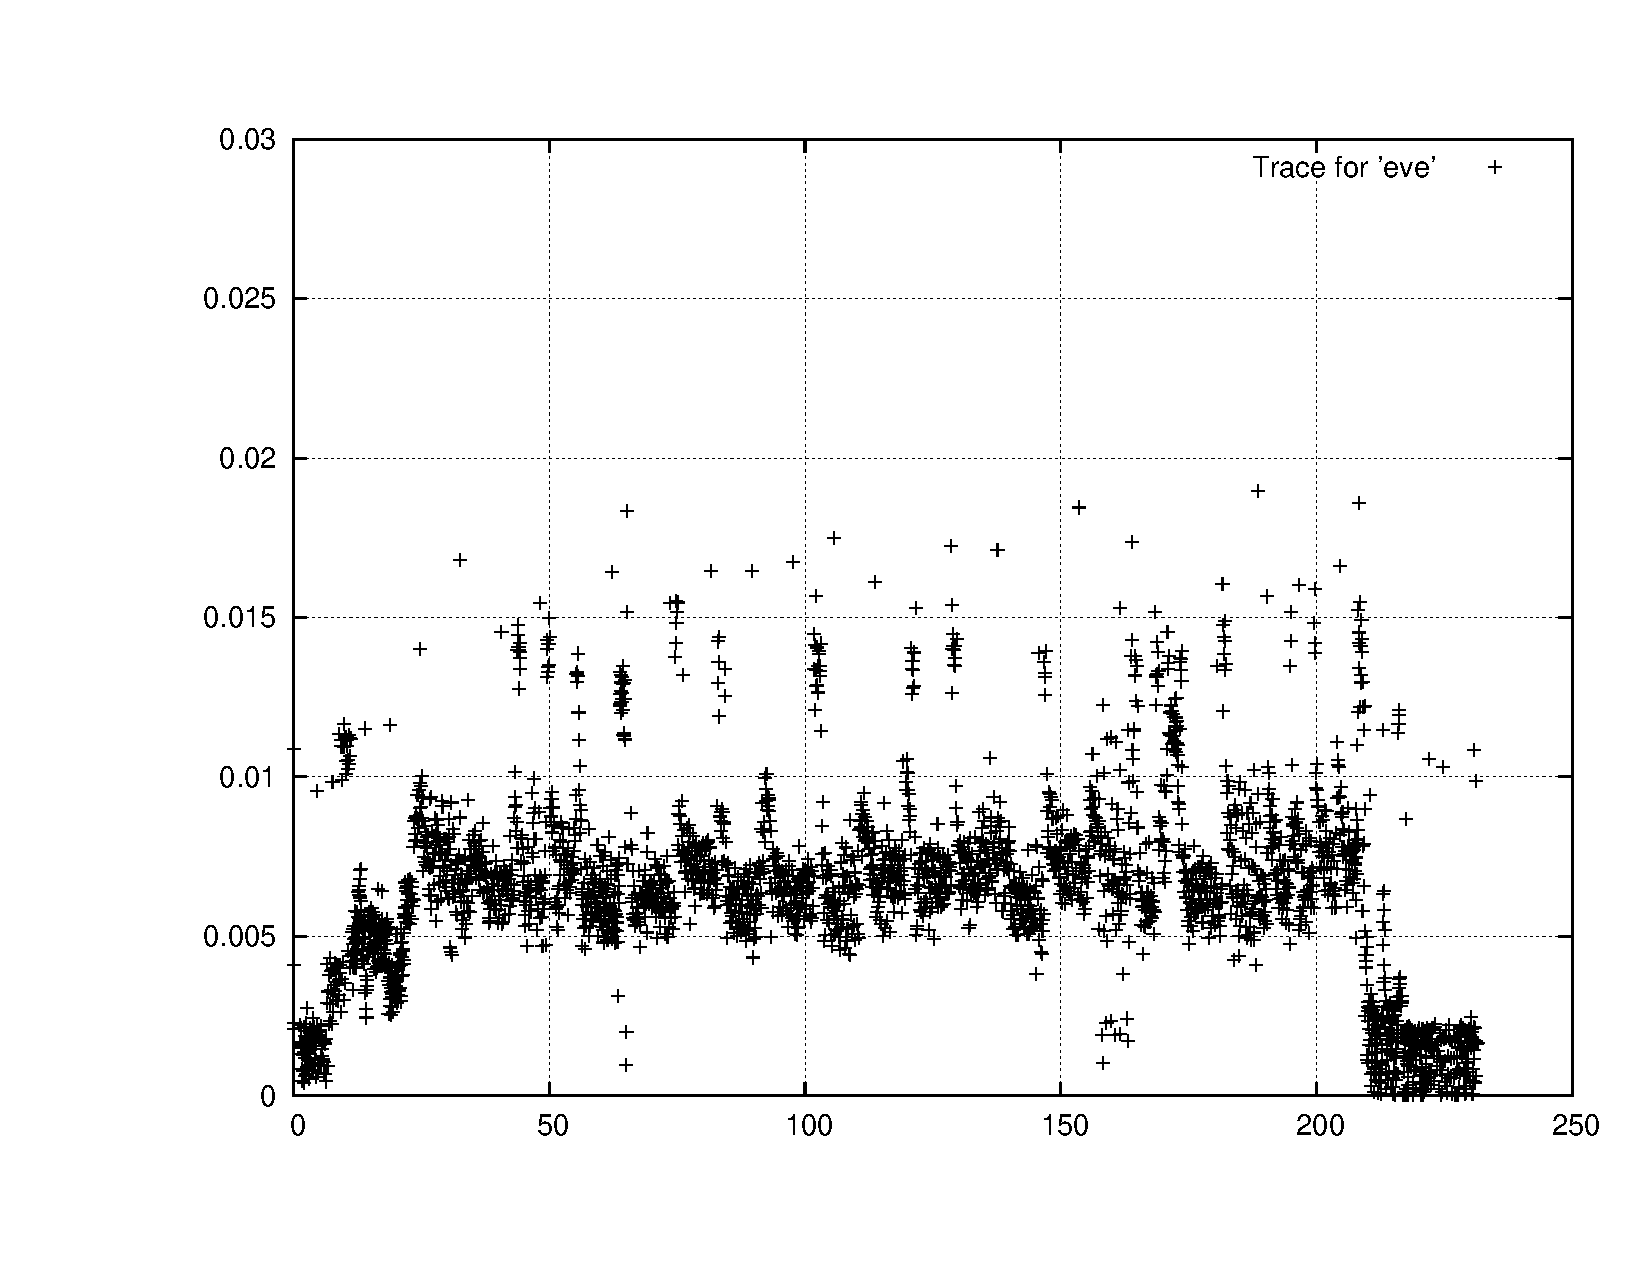
\includegraphics[scale=0.3]{trace-eve}
    \label{fig:plot-trace-eve}
  }
  \subfloat[Normally distributed execution costs over time.]{
    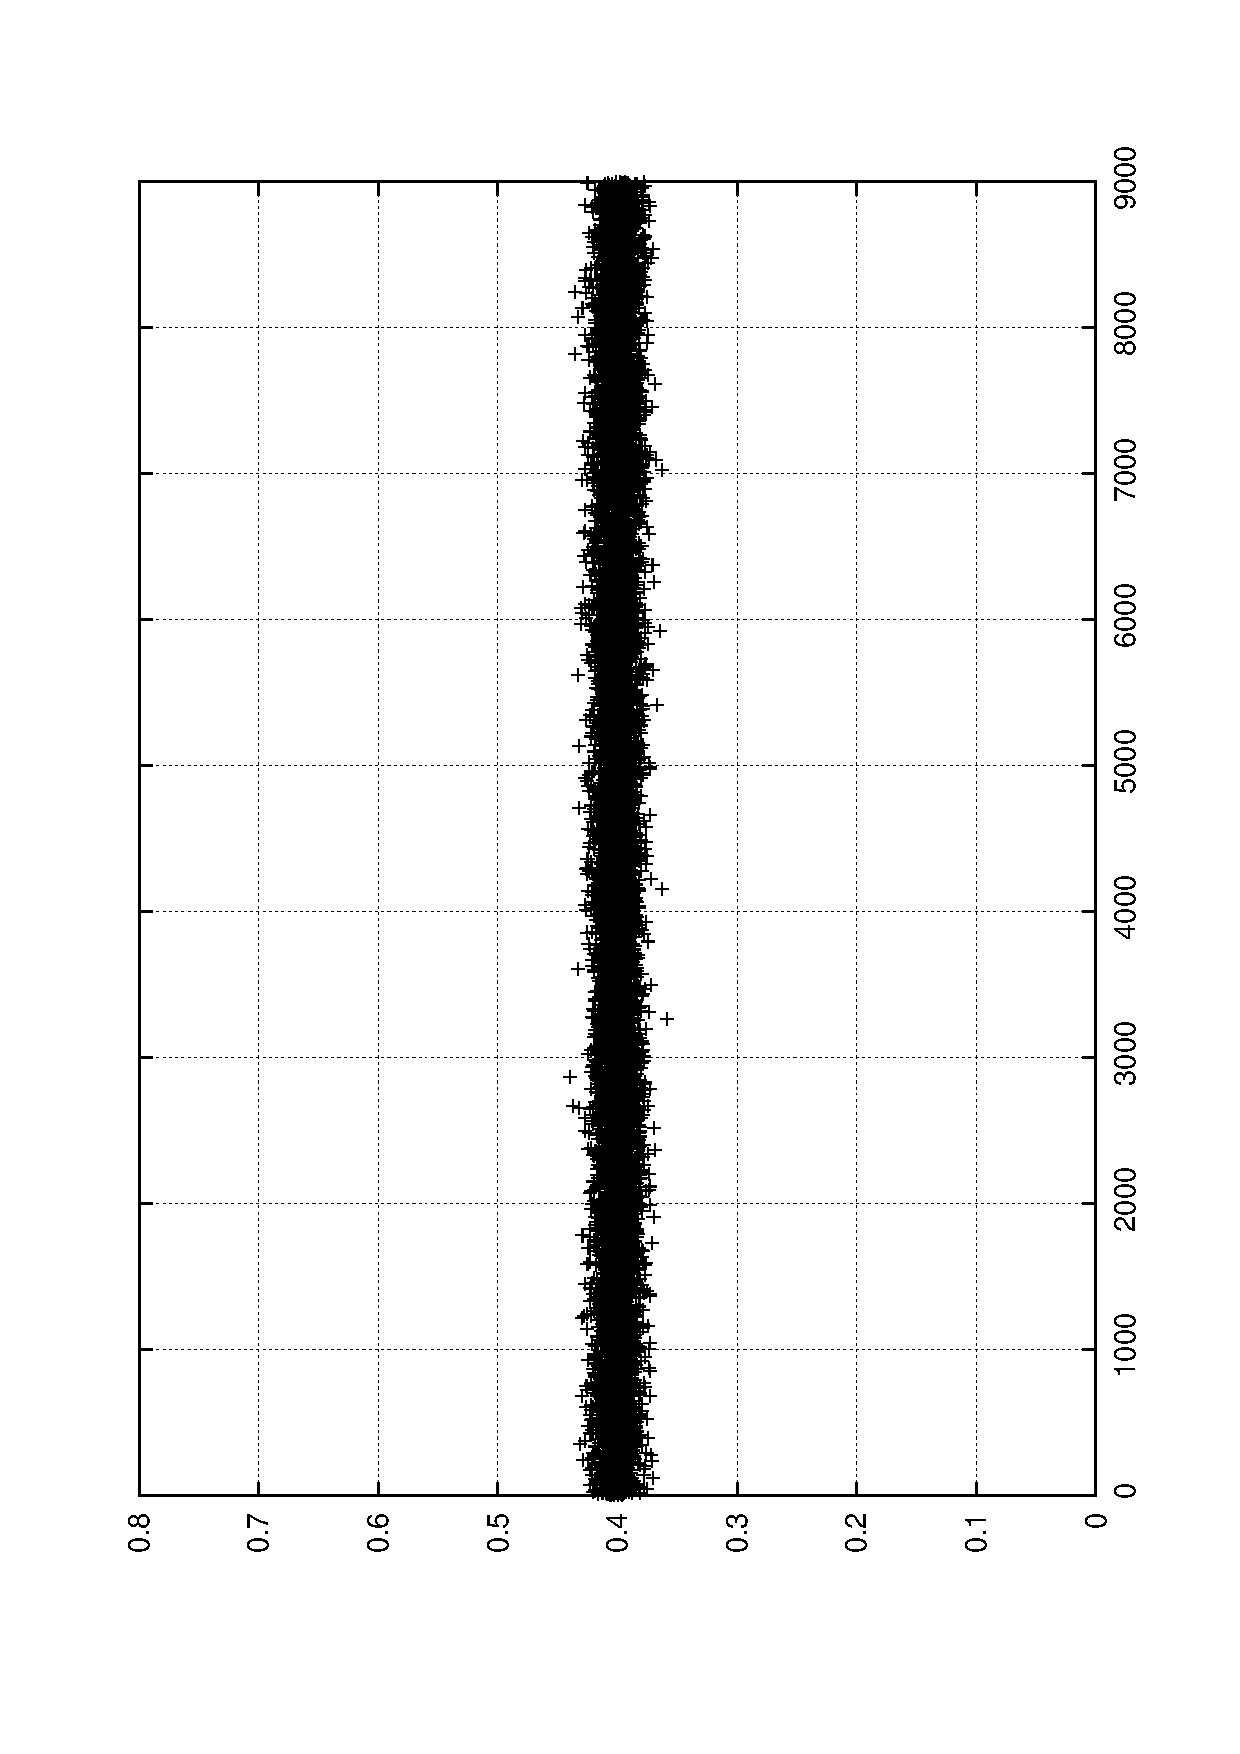
\includegraphics[scale=0.3]{trace-normal}
    \label{fig:plot-trace-normal}
  }
  \caption{Execution cost models used in our simulations.}
\end{figure*}

Not all these variables highlight any difference in whether hard or
soft reservation is better, and by how much. To study the actual
effects of a reservation model, we chose some performance metrics to study.

\subsection{Performance Metrics}
\label{sec:metrics}

In a soft real-time system the most important concern is maintaining a
good \textbf{response time} without wasting system resources or
prejudicating any hard real-time tasks present in the system
\cite{buttazzo05:soft}. This suggests that a good way to measure
performance in soft real-time systems is measuring the mean response
time of tasks in it. This is, on the other hand, rather naïve, since
there are many undesirable trade-offs one might make that reduce the
mean response time for tasks and yet make a system perform overall
worse. A simple example is that whenever tasks missing their deadlines
are discarded one can always reduce mean response time by discarding
all tasks with a sufficiently high cost. This clearly degrades the
overall system performance. For this reason we're interested also in
the mean \textbf{response interval}, which is the interval between two
successive completions of a task. If no deadlines are missed the mean
response interval should be near the period of the tasks, but whenever
tasks are discarded it should go up. We propose that the mean response
interval is a more robust estimator for the perceived performance of a
system than the mean response time.

One supposed difference between soft and hard reservation in CBS
servers is that, when using soft reservation, the server might pospone
its deadline indefinitely in a period of high load, making for a very
low responsivity afterwards. To gauge whether or not this is really a
problem we are also measuring the mean \textbf{delay} between a task's
arrival time and the time it starts executing. Also, to highlight any
perceived problems of soft reservation under this condition we use the
costs seen in figure \ref{fig:costs-trifasico}.

\begin{figure}[t]
  \centering
  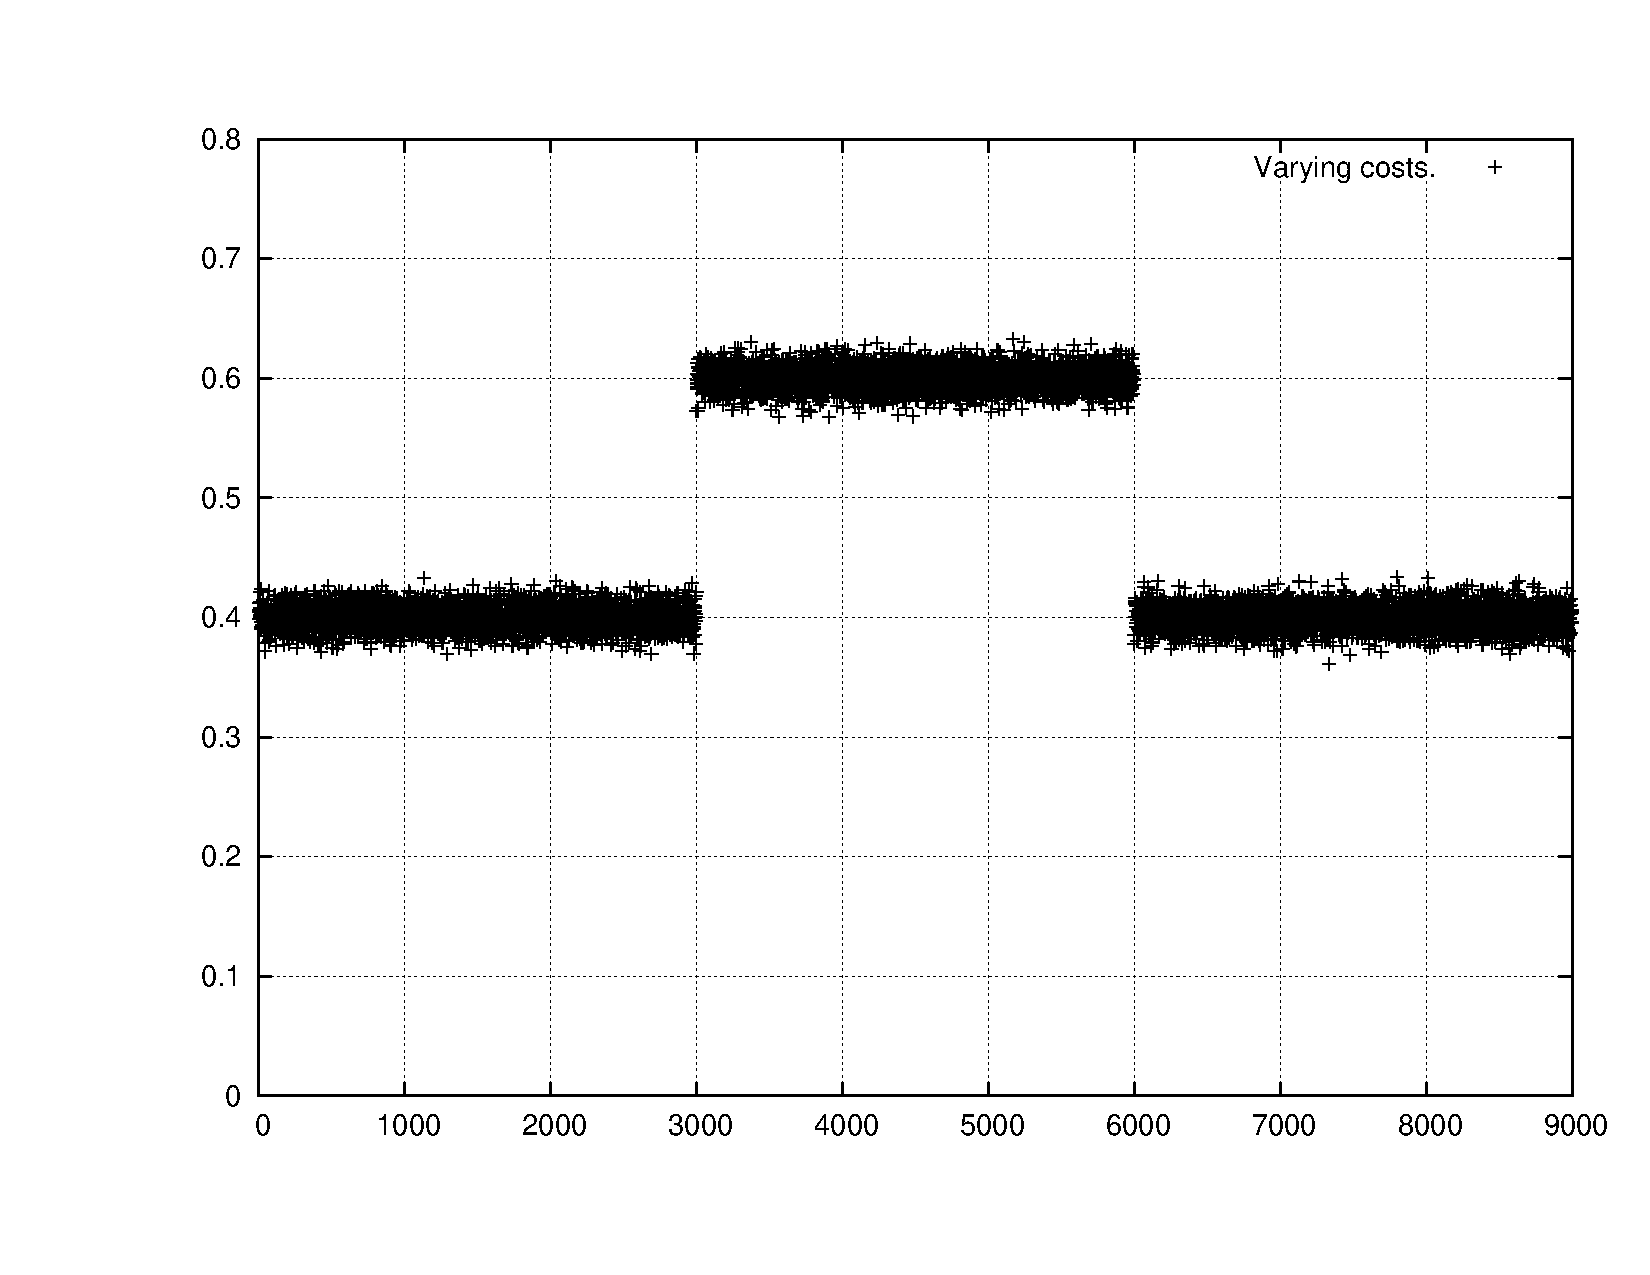
\includegraphics[scale=0.3]{trace-trifasico}
  \caption{Execution costs designed to postpone deadlines under soft reservation.}
  \label{fig:costs-trifasico}
\end{figure}

We also measure percentual of discarded tasks and mean lateness, when
applicable.

\section{Simulation Results}
\label{sec:simulation-results}

We found that not discarding expired tasks makes soft and hard
reservation completely equivalent. In the absence of system idle time,
also, both reservation schemes are equivalent. This suggests that in
systems that are expected to be overloaded or in systems where all
tasks must be run until completion there is no need to worry about
using either soft or hard reservation. Also, if the server load is
low, there is no difference, as there is no need for the soft
reservation mechanism to use any extra bandwidth. Summarizing, the
relevant scenarios are when
\begin{itemize}
\item tasks that have overrun their deadlines are discarded,
\item there is idle time in the system,
\item but the soft real-time server is overloaded.
\end{itemize}
This leaves room for wiggling the variance of execution costs and
specific characteristics of the the task set over time.

\begin{figure*}[t]
  \centering
  \subfloat[Soft reservation.]{
    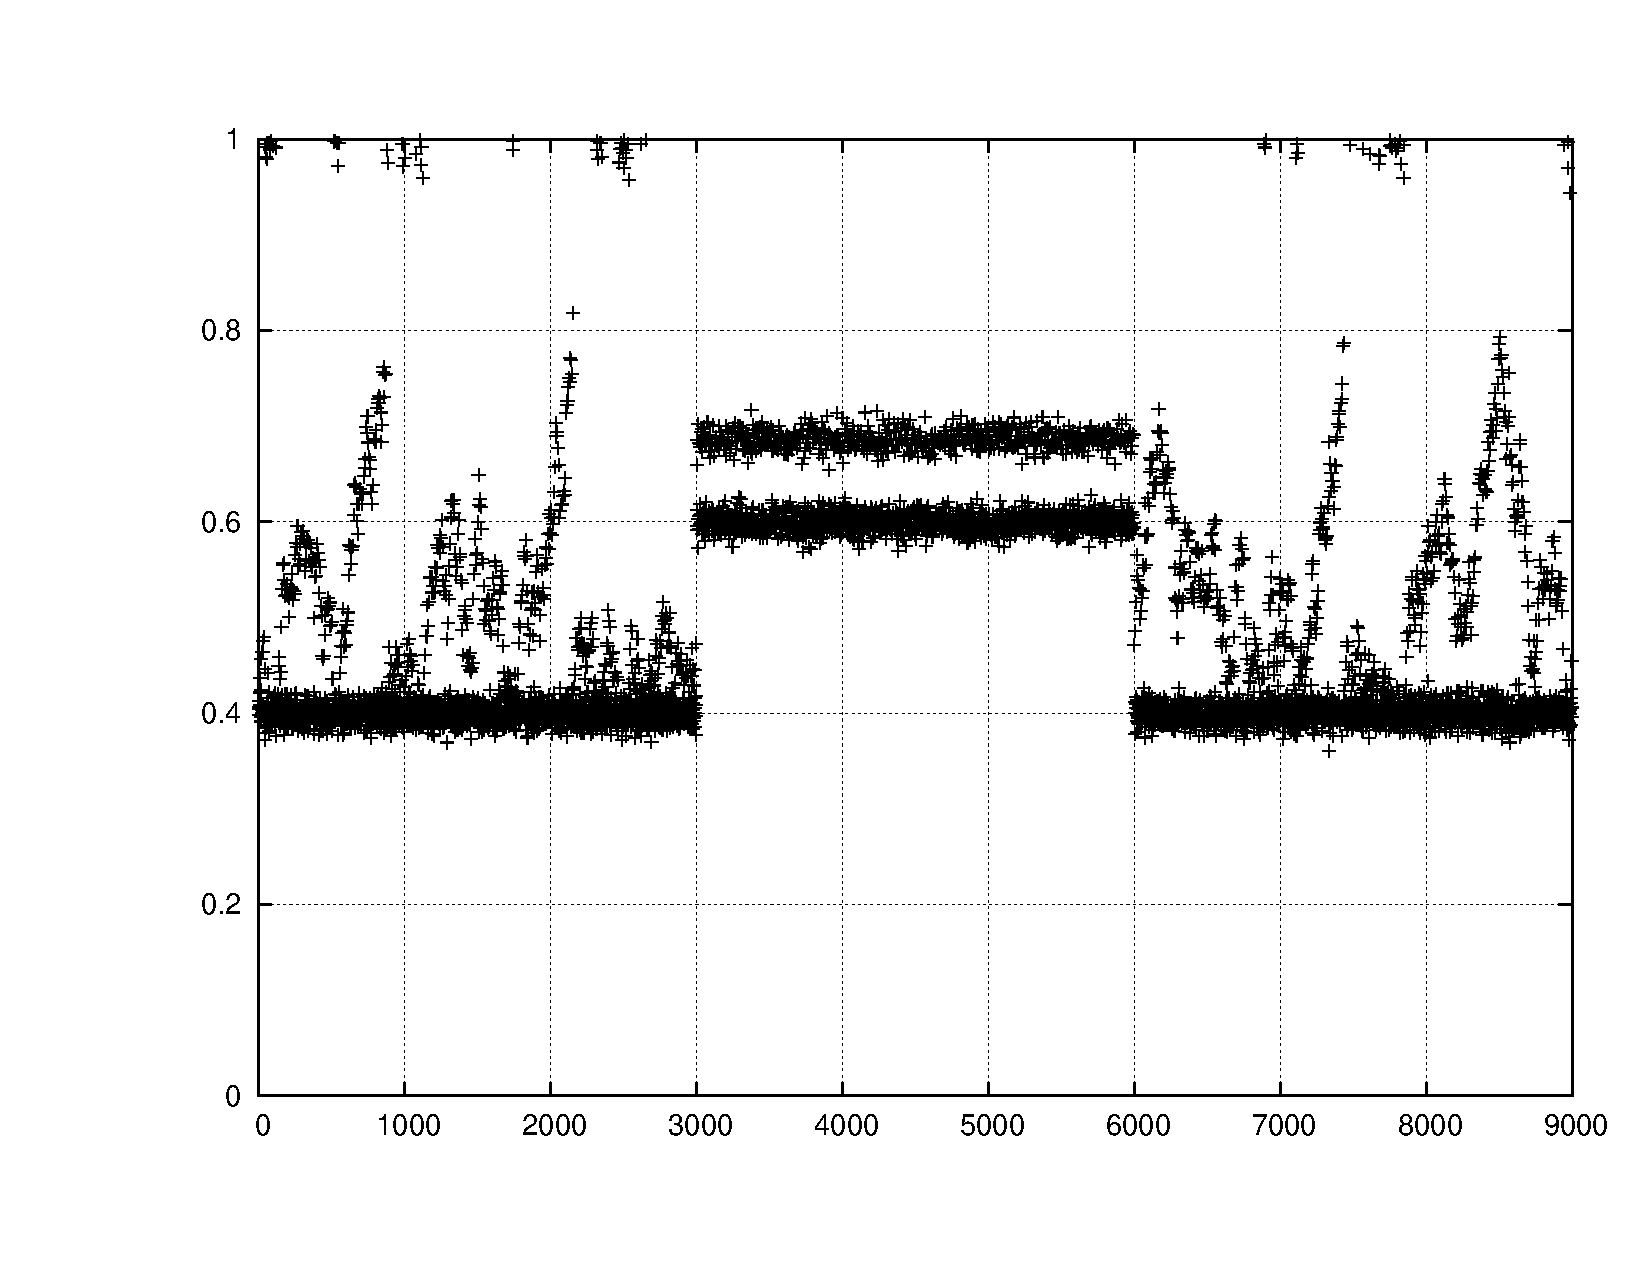
\includegraphics[scale=0.3]{trifasico-1}
    \label{fig:soft-trifasico}
  }
  \subfloat[Hard reservation.]{
    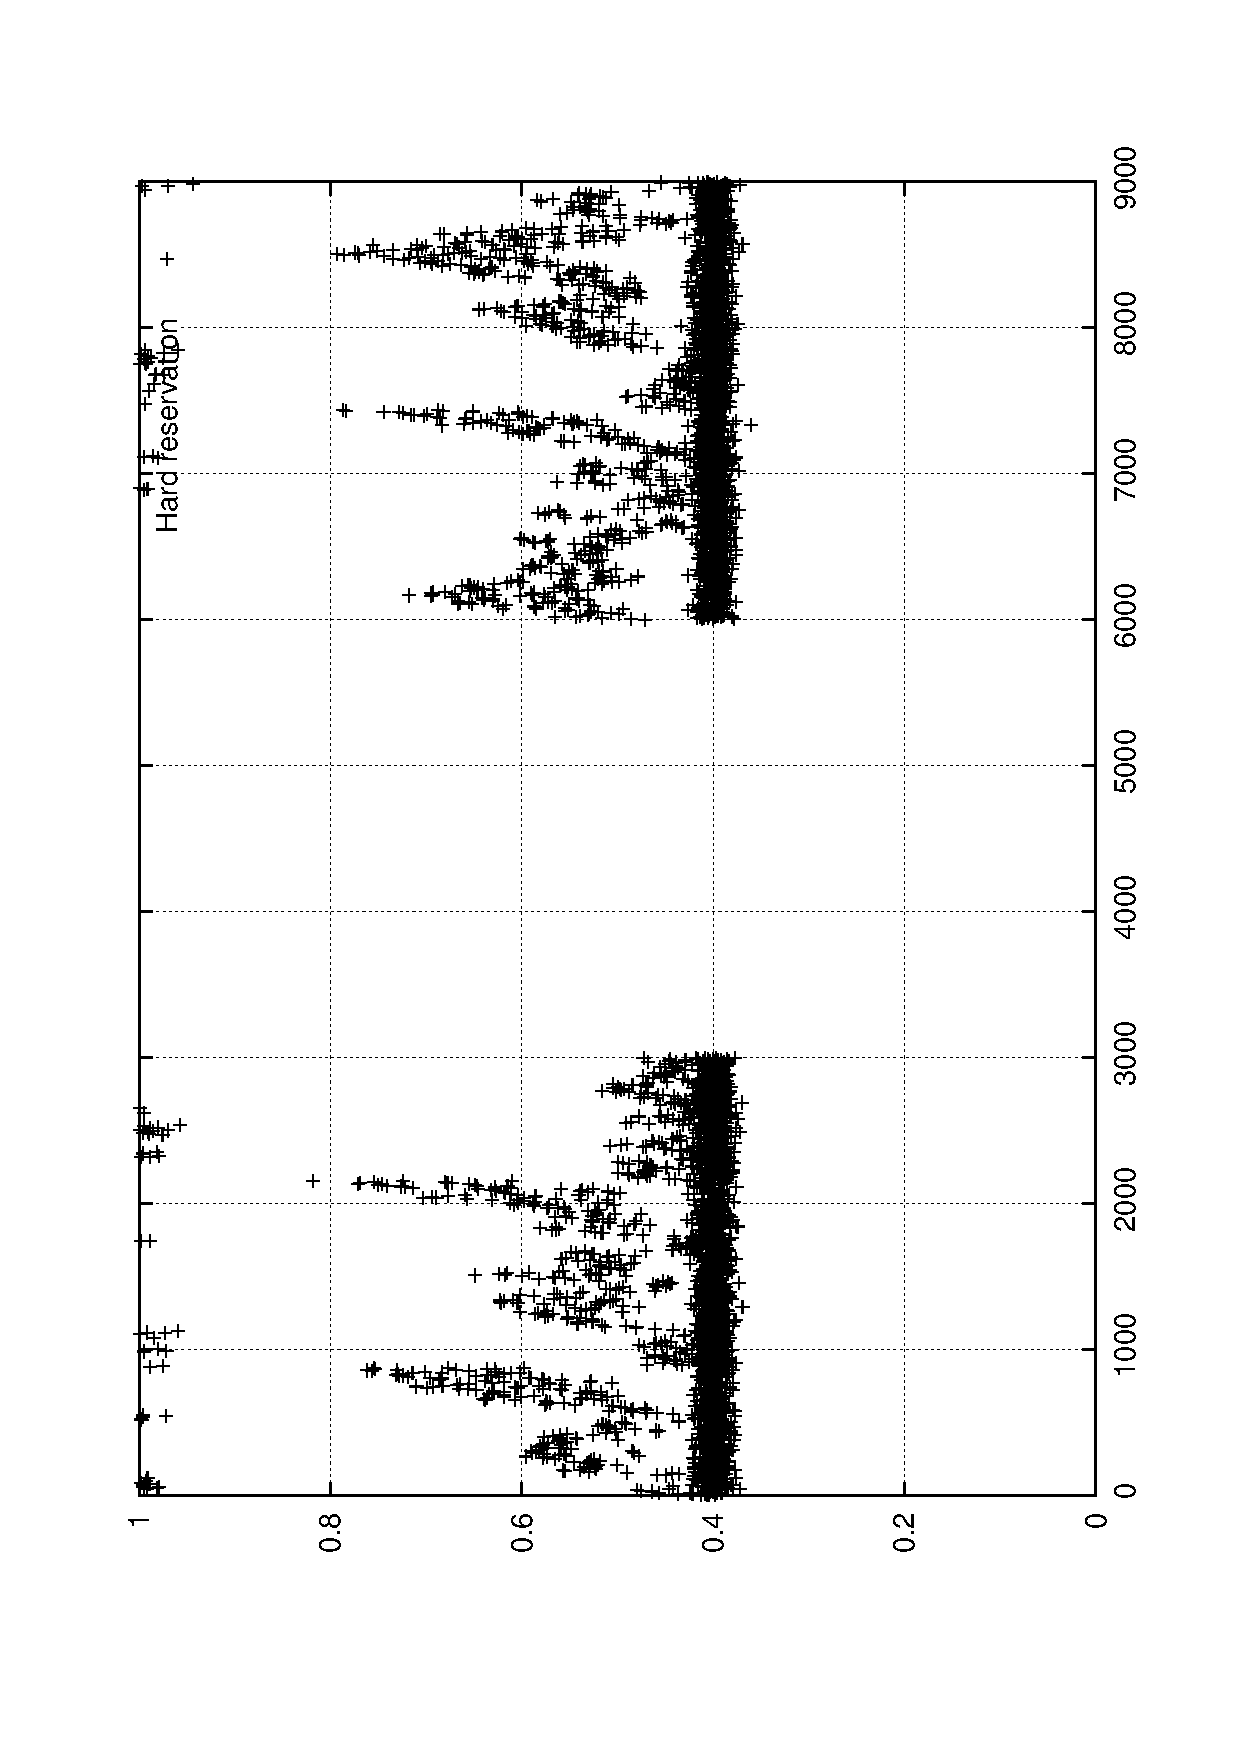
\includegraphics[scale=0.3]{trifasico-2}
    \label{fig:hard-trifasico}
  }
  \caption{Response times for the costs in figure
    \ref{fig:costs-trifasico}.}
  \label{fig:trifasico}
\end{figure*}

For the experiment with adaptivity, the results are in figure
\ref{fig:trifasico}. As can be seen, when the server is not under
heavy load both soft and hard reservation perform acceptably. On the
other hand, in the heavily loaded part only the soft reservation
server can use finish tasks that need more than its budget. As
expected, when the load comes back down there is no extra cost for the
soft reservation server, and its response times are equivalent to the
hard reservation ones.

\begin{figure*}[t]
  \centering
  \subfloat[Soft reservation.]{
    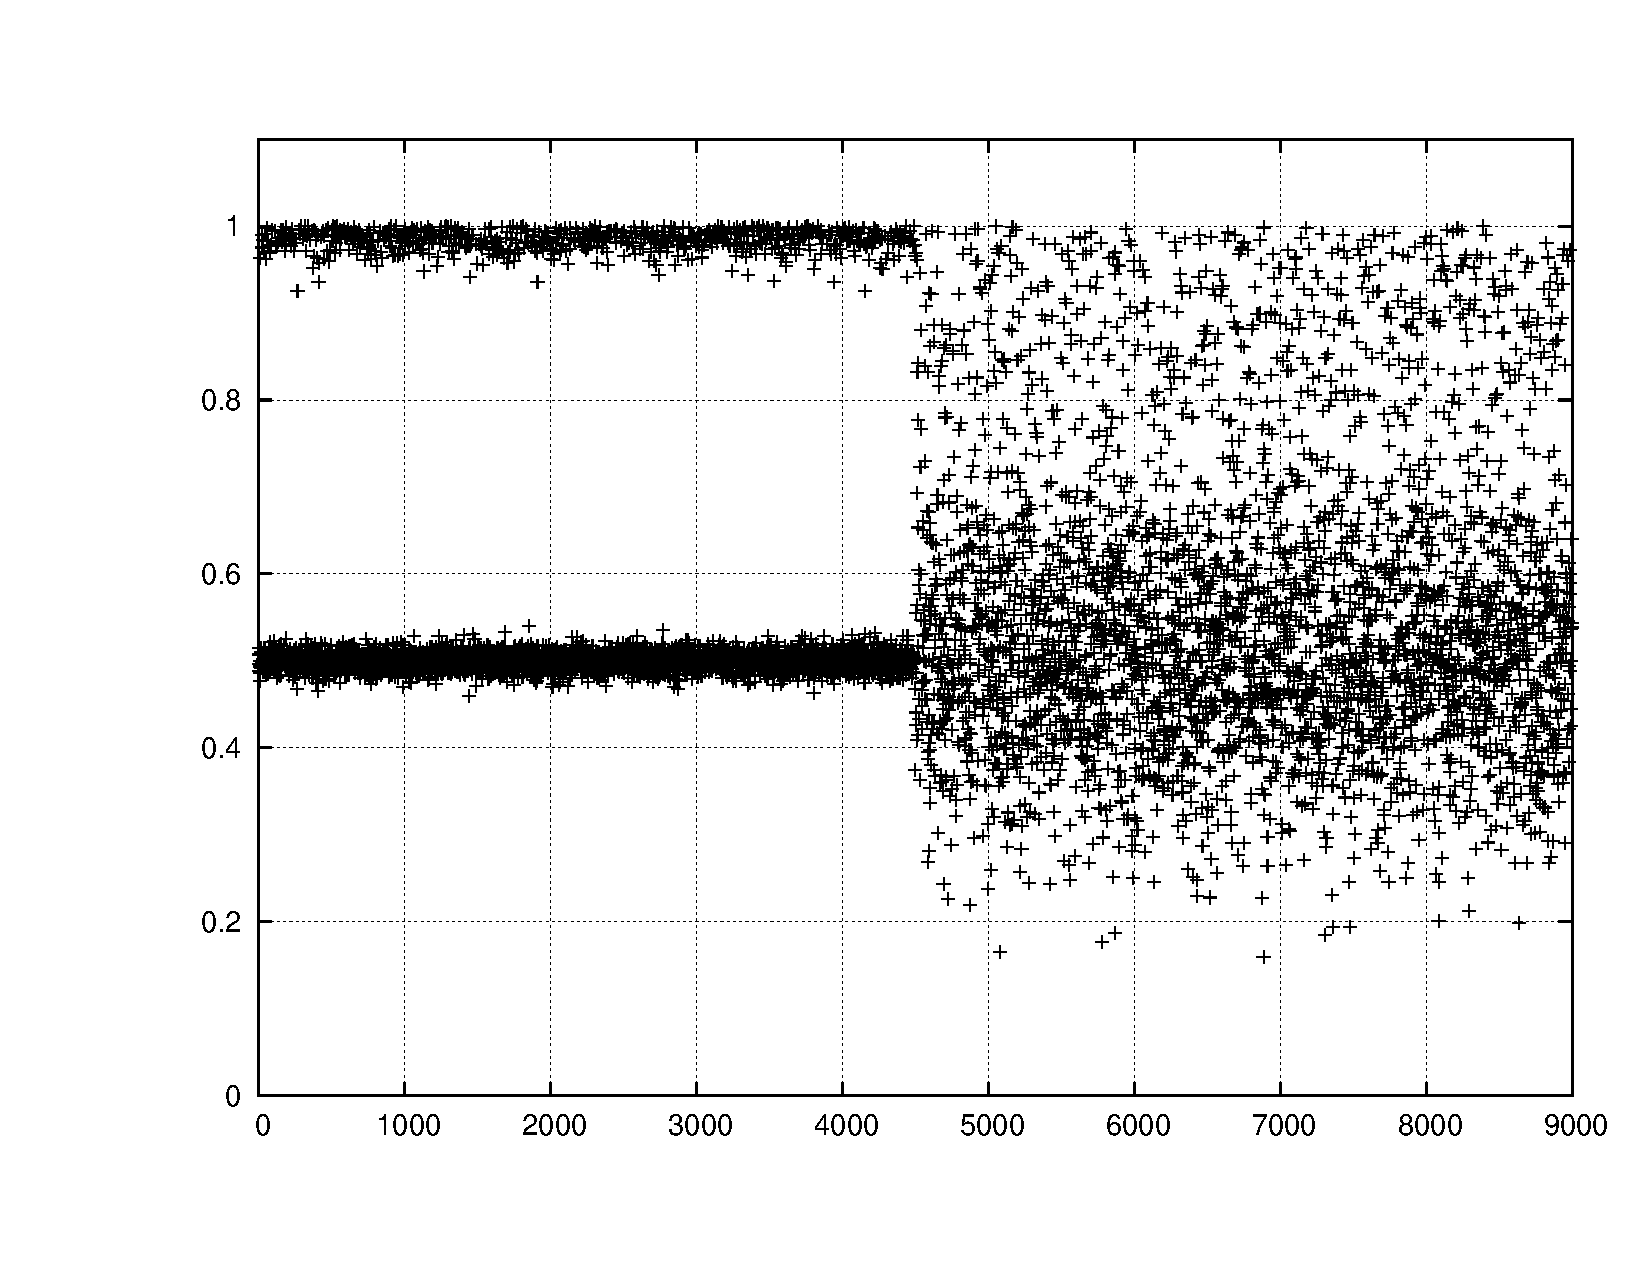
\includegraphics[scale=0.3]{variance-1}
    \label{fig:soft-variance}
  }
  \subfloat[Hard reservation.]{
    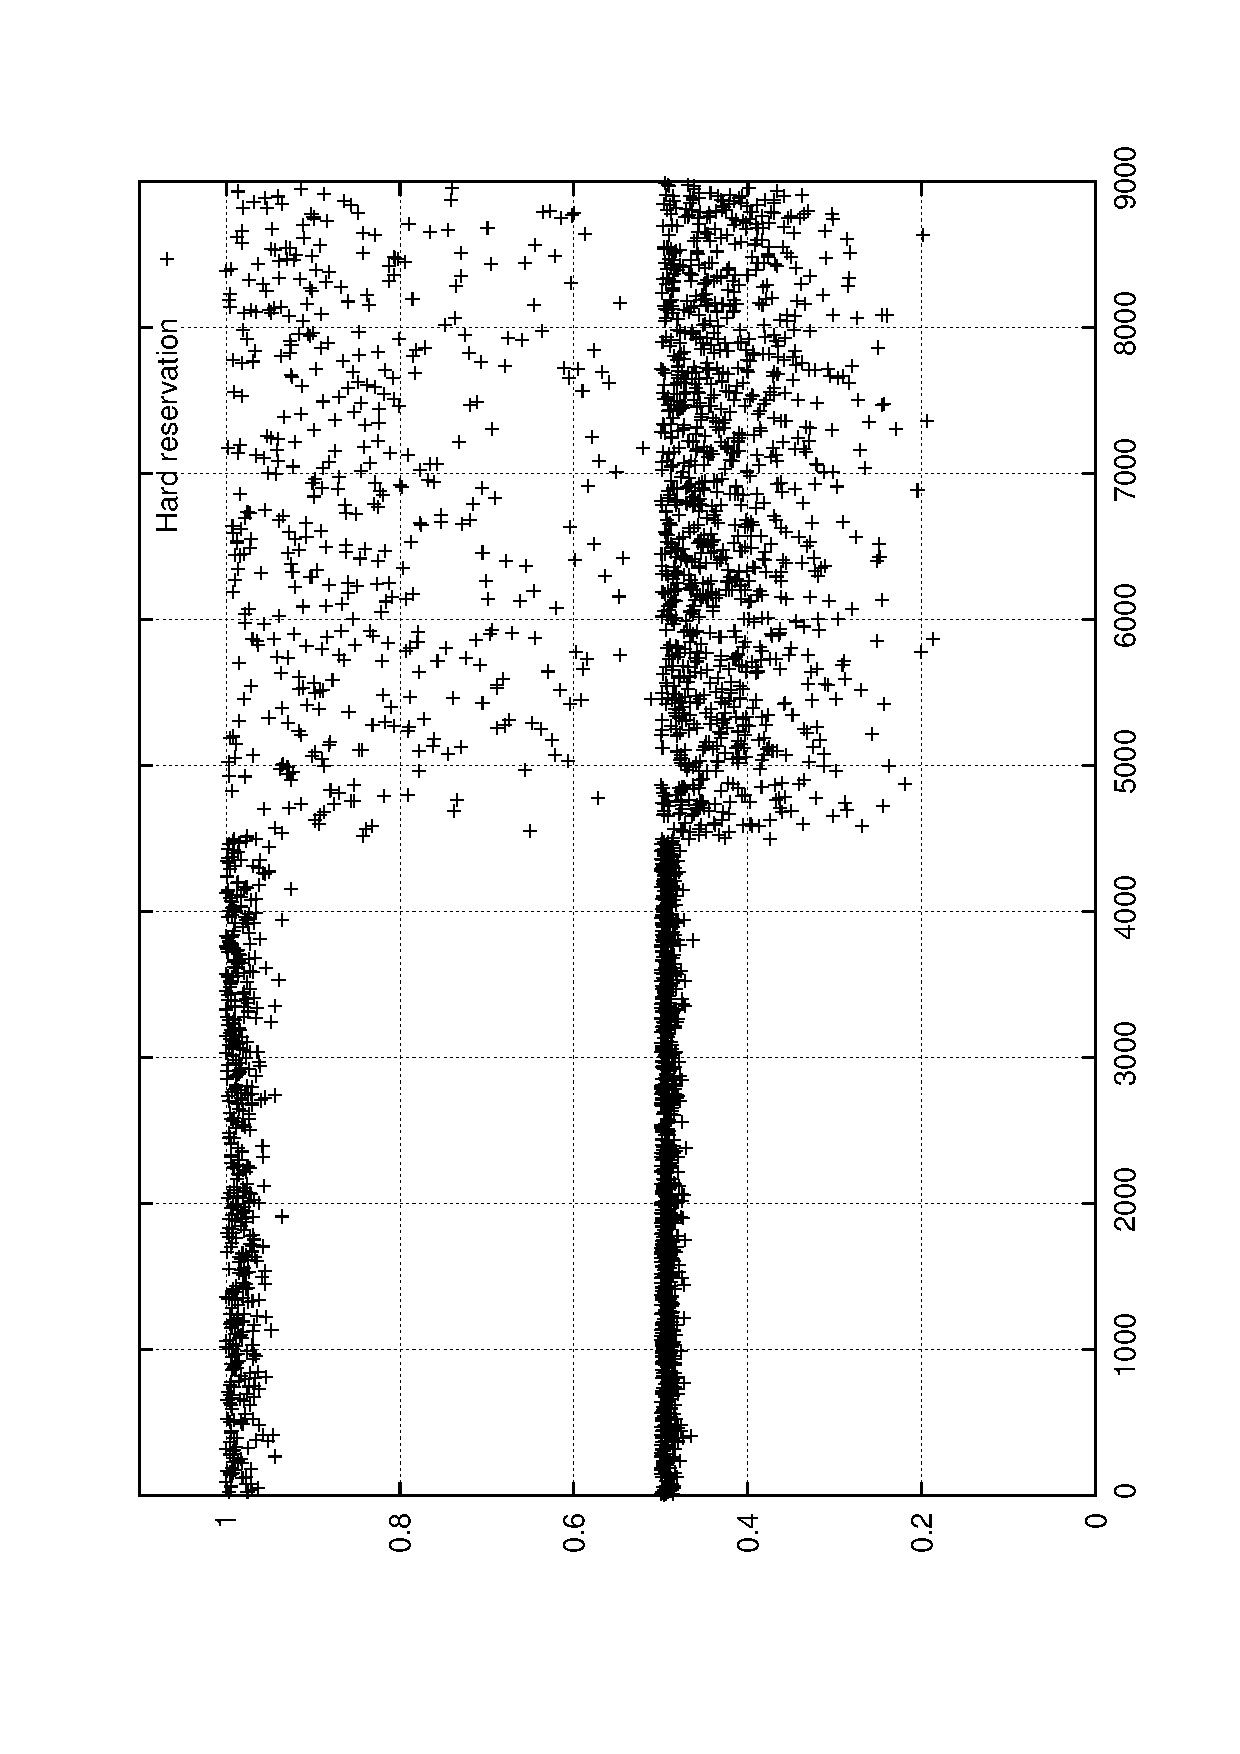
\includegraphics[scale=0.3]{variance-2}
    \label{fig:hard-variance}
  }
  \caption{Response times for the high variance case.}
  \label{fig:variance}
\end{figure*}


In the high variance experiment, the hard reservation server lost
59.39\% of the deadlines, while the soft reservation only lost
5.19\%. Figure \ref{fig:variance} shows the response times for this
experiment.

As can be seen in figures \nota{colocar as figuras}, soft reservation
usually outperforms hard reservation, having a smaller average
response time as well as a smaller worst-case response time, a shorter
delay between task arrival and start of execution, and a more uniform
interval between successive task terminations. Aside from the obvious
capacity of using extra free-time in a soft reservation framework,
some counter-intuitive properties, such as dealing better with
out-of-phase tasks, have been observed.

\section{Conclusion}
\label{sec:conclusion}



\bibliographystyle{latex8}
\bibliography{bib}
\end{document}
